\chapter{Background and Related Work}
\label{cha:background}
In chapter \ref{cha:intro}, there is a brief introduction about cloud computing.
To elaborate, three common cloud delivery models have become widely established and formalized:
Infrastructure-as-a-Service (IaaS), Platform-as-a-Service (PaaS), Software-as-a-Service (SaaS).
People may also refer to these classifications as: Cloud types, Cloud models, service models,
paradigms or delivery models.

There are also four deployment models\cite{CloudModel}: Public, Private, Hybrid and Community.

Public cloud: The cloud infrastructure is provisioned for open use by the general public. It may be owned, managed, and operated by a business, academic, or government organization, or some combination of them. It exists on the premises of the cloud provider. 

Private cloud: The cloud infrastructure is provisioned for exclusive use by a single organization comprising multiple consumers (e.g., business units). It may be owned, managed, and operated by the organization, a third party, or some combination of them, and it may exist on or off premises.  

Hybrid cloud: The cloud infrastructure is a composition of two or more distinct cloud infrastructures (private, community, or public) that remain unique entities, but are bound together by standardized or proprietary technology that enables data and application portability (e.g., cloud bursting for load balancing between clouds).

Community cloud: The cloud infrastructure is provisioned for exclusive use by a specific community of consumers from organizations that have shared concerns (e.g., mission, security requirements, policy, and compliance considerations). It may be owned, managed, and operated by one or more of the organizations in the community, a third party, or some combination of them, and it may exist on or off premises.


\section{Cloud Computing Paradigm}
The Cloud computing paradigm is shifting computing from in-house managed
hardware and software resources to virtualized Cloud-hosted
services. Cloud computing assembles large networks of
virtualized services: hardware resources (CPU, storage, and
network) and software resources (e.g., web server, databases,
message queuing systems, monitoring systems.). 

Cloud service types can be abstracted into three layers: Software as
a Service (SaaS), Platform as a Service (PaaS), and
Infrastructure as a Service (IaaS). Hardware and software
resources form the basis for delivering IaaS and PaaS. The
top layer focuses on application services by making
use of services provided by the lower layers. PaaS/SaaS
services are often developed and provided by third party
service providers who are different from the IaaS providers.

Cloud providers including Google Cloud Platform \cite{google_cloud},
Amazon Web Services (AWS) \cite{aws}, Microsoft Azure \cite{azure}, 
Rackspace \cite{Rackspace},
Alibaba Cloud \cite{Alibaba}, FlexiScale \cite{FlexiScale}, 
DataCentred \cite{DataCentred}, IBM \cite{IBMSoftLayer} and others
give users the options to deploy their applications over a pool
of virtually infinite services with practically no capital
investment and with modest operating costs proportional to
the actual use. Elasticity, cost benefits and abundance of
resources motivate many organizations to migrate their
enterprise applications to the Cloud. Although the Cloud offers
the opportunity to focus on revenue growth and innovation,
decision makers (e.g., CIOs, scientists, developers,
engineers, etc.) are faced with the complexity of choosing
the right service delivery model for composite applications
and infrastructure across private, public, and hybrid Clouds.

In a cloud computing model, users access services according
to their requirements without the need to know where the
services are hosted or how they are delivered. 
A large number of information technology vendors claim to offer applications, storage,
and computation resources as cloud hosting services. As a
result, an exceeding number of competing services are available for
users to choose from, in such context, the migration of applications 
(e.g., multi-layered enterprise applications, scientific experiments, 
video-ondemand streaming applications, etc.) to the Cloud
demands selecting the best mix of services across multiple
layers (e.g., IaaS, PaaS, and SaaS) from an abundance of
possibilities. Any such Cloud service selection decision has
to cater for a number of conflicting criteria while ensuring that 
Quality of Service (QoS) requirements are met. For example, minimizing cost,
network latency, while maximizing throughput, storage space, CPU power (for analytical
programs to process more job or do it faster), RAM (bigger buffer size), etc.
QoS requirements for different applications also are varied. 
For example, scientific experiments need to meet deadlines, thus time/duration are constrained. 
On the other hand, video-on-demand streaming application need to satisfy streaming latency, resolution requirements.

Naturally, it is challenging for users to
select the right services that meet their QoS requirements in the
service cycle from selection and deployment to orchestration
(e.g., determining an optimal web service when making service
selection, identifying suitable virtual machine (VM) servers for
deploying web service instances, etc.). Effective service
recommendation techniques are becoming important to help
users (including developers) in their decision-making processes
for critical application developments and deployments. 

\section{Cloud Computing Scope}

Figure \ref{fig:cloud_computing} illustrates the relationship between Cloud
and \textbf{web service}. Web service generally does not include IaaS.

\begin{figure}[ht]
  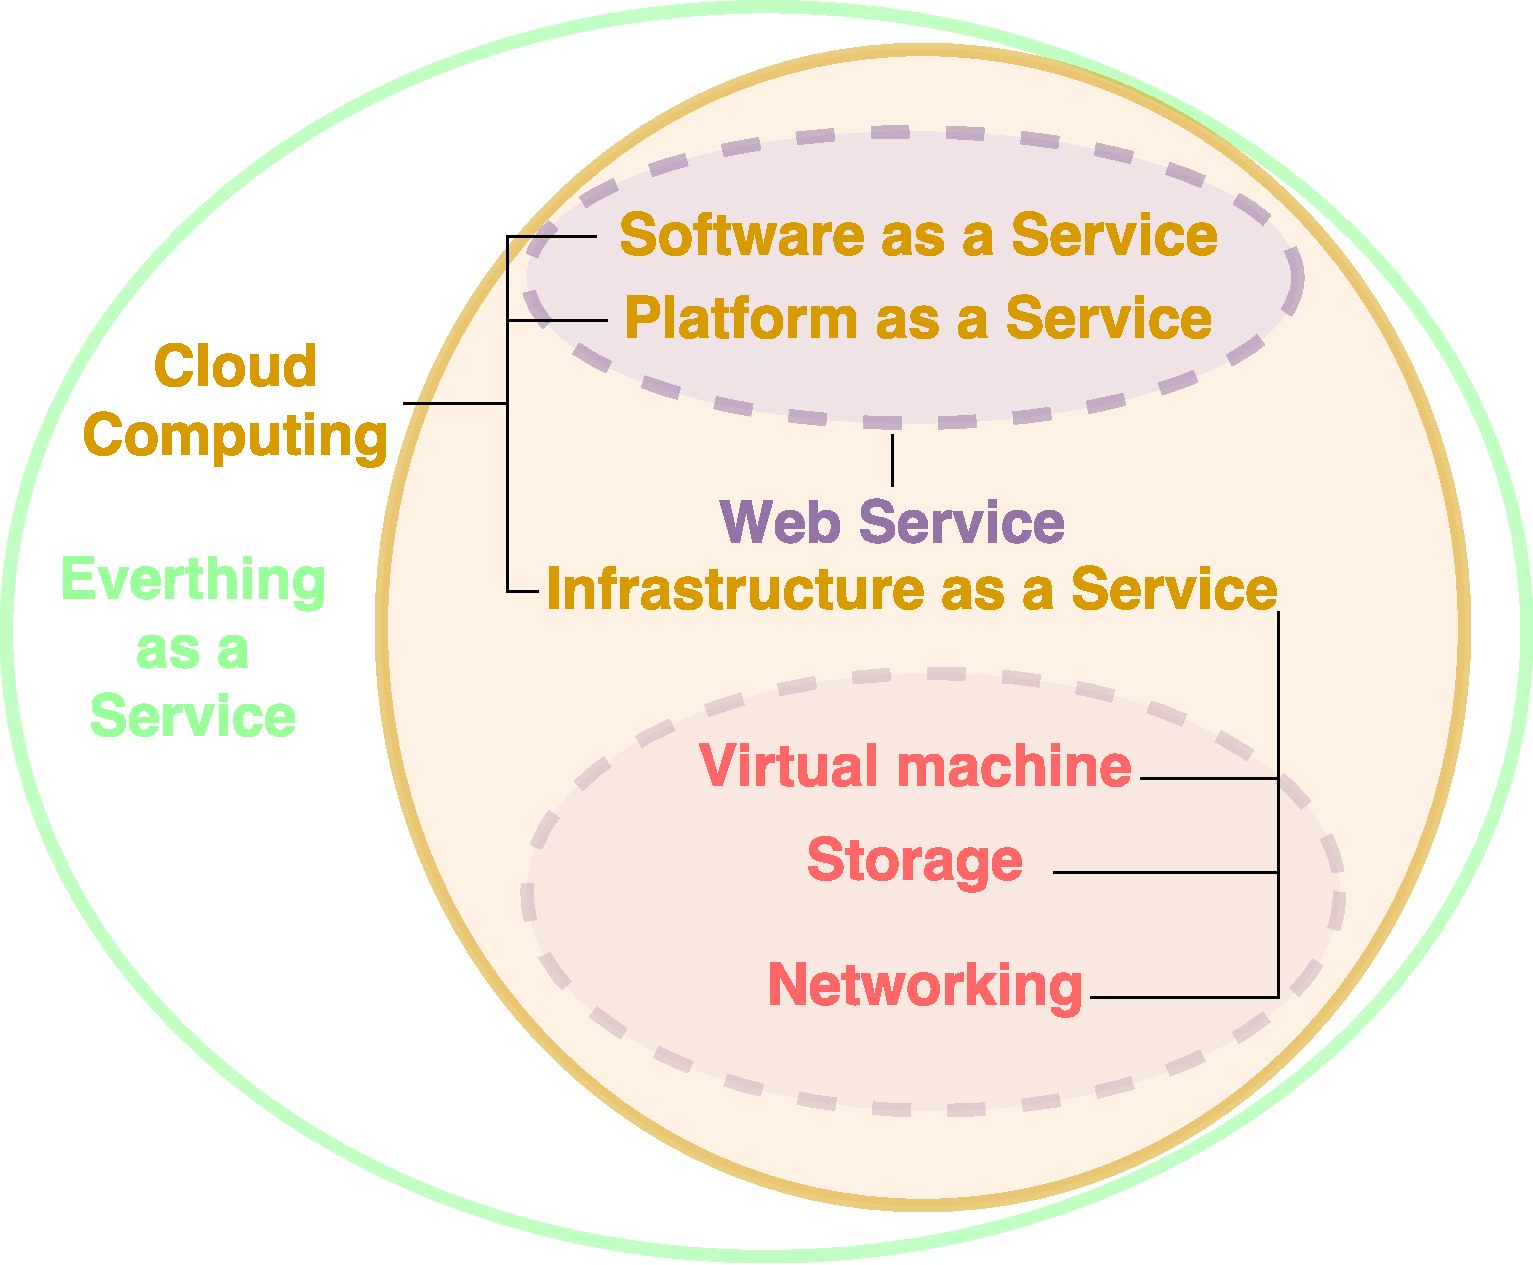
\includegraphics[width=\textwidth]{cloud_computing_venn.pdf}
  \caption{Cloud Computing.}
  \label{fig:cloud_computing}
\end{figure}

Cloud computing differs from \textbf{traditional web hosting},
mainly because of the application of visualization layer.
Visualization technology offers greater freedom resulting a
much higher scalability, and enables finer grained billing model (Pay as You Go).
see Chapter \ref{cha:system} for more information.

\textbf{Grid computing} is the collection of computer resources from multiple locations to reach a common goal. The grid can be thought of as a distributed system with non-interactive workloads that involve a large number of files \cite{grid_computing}.
In comparison, Cloud computing has more generic use cases, applicable to handle large, small or dynamic workload.

\section{Cloud Concepts}

\subsection{Virtualization}
Virtualization technique was developed in late 1990s and is different from simulation and emulation.
Virtualization employs techniques used to create instances of an environment, as opposed to simulation, which models the environment; or emulation, which replicates the target environment such as certain kind of virtual machine environment. Full virtualization requires that every salient feature of the hardware be reflected into one of several virtual machines – including the full instruction set, input/output operations, interrupts, memory access, and whatever other elements are used by the software that runs on the bare machine, and that is intended to run in a virtual machine \cite{virtualization}.

\subsection{Hypervisor}

A hypervisor is computer software, firmware that creates and runs virtual machines. A computer on which a hypervisor runs one or more virtual machines is called a host machine, and each virtual machine is called a guest machine. The hypervisor presents the guest operating systems with a virtual operating platform and manages the execution of the guest operating systems. Multiple instances of a variety of operating systems may share the virtualized hardware resources: for example, Linux, Windows, and Mac OS instances can all run on a single physical x86 machine \cite{hypervisor}. See table \ref{table:hypervisor_types} for types and examples of hypervisor.

\begin{table}
    \begin{tabular}{ p{70mm} | p{70mm} }
        \hline
        \multicolumn{2}{c}{Types of hypervisor} \\
        \hline
        Native or Bare-metal & Hosted \\
        \hline
            Run directly on the host's hardware.& 
            Run on a conventional operating system (OS)\\
        \hline
            These hypervisors run directly on the host's hardware to control the hardware and to manage guest operating systems. For this reason, they are sometimes called bare metal hypervisors.& 
            These hypervisors run on a conventional OS just as other computer programs do. A guest operating system runs as a process on the host. These hypervisors abstract guest operating systems from the host operating system.   \\
        \hline
        \multicolumn{2}{c}{Examples} \\
        \hline
            Xen \cite{Xen}, Microsoft Hyper-V \cite{Hyper-V}, VMware ESX \cite{VMware_ESXi} & 
            VMware Workstation \cite{VMware_Workstation}, VMware Player, VirtualBox \cite{VirtualBox} \\
        \hline
    \end{tabular}
    \caption{Types of hypervisor}
    \label{table:hypervisor_types}
\end{table}

\subsection{Containerization}

Operating-system-level virtualization, also known as containerization, refers to an operating system feature in which the kernel allows the existence of multiple isolated user-space instances. Such instances, called containers, may look like real computers from the point of view of programs running in them. 
A computer program running on an ordinary person's computer's operating system can see all resources (connected devices, files and folders, network shares, CPU power, quantifiable hardware capabilities) of that computer. However, programs running inside a container can only see the container's contents and devices assigned to the container \cite{containerization}.
An example implementation is Docker \cite{docker}.

\subsection{Everything as a Service}
Everything as a service (EaaS, XaaS, *aaS) is initially a concept of being able to call up re-usable, fine-grained software components across a network. The most common and successful example is software as a service, but the term as a service has been associated and used with many core components of cloud computing including communication, infrastructure, data and platforms \cite{XaaS}.

As the term getting more popular, a number of vendors including Google, Microsoft, Hewlett Packard, Amazon have been associated with the "everything as a service" trend, i.e. machine learning as a service, mobile backend as a service, mechanical turk (human as a service), security and testing as a service.

XaaS is not only limited to online services. Bricks-and-mortar businesses are also being transformed through digital connectivity. Transportation-as-a-service is being fulfilled by companies like Uber and Lyft; grocery-as-a-service is being offered by chains such as Safeway and Whole Foods; and accommodation-as-a-service is a lodging rental service provided by Airbnb. This is just the tip of the iceberg with many more on their way \cite{XaaS_beyond}.

\section{Ontological Knowledge Representation}
Many industries (i.e. smart factories, business analytics) are
becoming increasingly dependent on complex automatic software systems for tasks like resource allocation, business decision making, etc.
For example, to make decentralized decisions, those systems need to cooperate with each other as well as with humans.
However, those systems typically access data from different models.
These information models have been independently developed in different (often incompatible) formats using different types of proprietary software; furthermore, they may not come with a well-defined semantics, and their specification can be ambiguous.
As a result, model development, maintenance, and integration, as well as data exchange and sharing pose major challenges in practice
\cite{CapturingIndustrialInformationWithOntologies}.

As a result, adoption of semantic technologies has been welcomed in many large companies such as in Google, Facebook, IBM \cite{SemanticTechnologiesInIBM}
and Siemens \cite{CapturingIndustrialInformationWithOntologies}.
For example, OWL 2 ontologies are often used to capture the conceptual information models.
OWL 2 is a rich and flexible modeling language. It not only comes with an
unambiguous, standardized, semantics, but also with a wide range of tools that can be used to
develop, validate, integrate, and reason with such models.
Data can be stored in RDF triplestores and effectively queried in conjunction with the available ontologies.
RDF is a standard model for data interchange on the Web.
RDF has features that facilitate data merging even if the underlying schemas differ,
and it specifically supports the evolution of schemas over time
without requiring all data consumers to be changed \cite{RDF}.
Moreover, legacy and other data that must remain in its original format can be virtualised as RDF using ontologies.

\subsection{Terminology, Taxonomy and Ontology}
Terminology is a system or collection of words. The system is managed to make content more consistent and standardized. Terminology helps improve readability, translation, and brand perception \cite{TaxonomyVSTerminology}.

A taxonomy is a way to classify words into hierarchical groups. The biggest use of a taxonomy is for search.
A taxonomy defines groups of words. It can be multi-layered or flat \cite{TaxonomyVSTerminology}.

An ontology describes a concept both by its position in a hierarchy and its relationships to other concepts. The richness of the relationships described in an ontology is what makes more powerful for modeling complex systems \cite{OntologyHasRicherRelationshipThanTaxonomy}.

In computer-science Taxonomy has been adopted to name trees of generalization-specialization relation. In ontologies can be build over any kind of relationships, including generalization-specialization and many other.
Taxonomies and ontologies usually concern terms but they are not limited to such. In terms of graph theory, taxonomies are trees, and ontologies are graphs or hyper-graphs, where edges are build from many different relations. Those relation could have any properties according to set theory \cite{taxonomiesRtreesOntologiesRgraphs}.

\subsection{Ontology versus Database}

For those who are familiar with database, ontology axioms are like DB schema.
In database, schema describes structure of and constraints on data.
Ontology facts are like DB data, they are consistent with schema constraints \cite{OntologyLanguageTool2}.
For differences, see table \ref{table:ontology_vs_database}. 
The given examples are expressed with Description Logic, see Section \ref{sec:DL} for more details.

\begin{longtable}[ht]{| p{65mm} | p{65mm} |} 
\hline
\rowcolor{orange} Database & Ontology\\
\hline
\rowcolor{green} Closed word assumption (CWA) & Open world assumption (OWA)\\ 
Missing information treated as false & Missing information treated as unknown\\
\hline
\rowcolor{lightgray} \multicolumn{2}{|c|}{For example, we have the following facts/data:}\\
\rowcolor{lightgray} \multicolumn{2}{|c|}{HarryPotter hasFriend RonWeasley}\\
\rowcolor{lightgray} \multicolumn{2}{|c|}{HarryPotter hasFriend HermioneGranger}\\
\hline
\multicolumn{2}{|c|}{Query: Is Draco Malfoy a friend of HarryPotter?}\\
\hline
DB: No & Ontology: Don’t Know (didn’t say Draco was not Harry’s friend)\\
\hline
\rowcolor{green} Unique name assumption (UNA) & No UNA \\ 
Each individual has a single unique name & Individuals may have more than one name\\
\hline
\multicolumn{2}{|c|}{How many friends does Harry Potter have?}\\
\hline
DB: 2 & Ontology: at least 1 (Ron and Hermione may be 2 names for same person)\\
\hline
\rowcolor{green} Schema behaves as constraints on structure of data & Ontology axioms behave like implications (inference rules) \\ 
\hline
\rowcolor{lightgray} \multicolumn{2}{|c|}{For example, if we try to add new facts/data:}\\
\rowcolor{lightgray} \multicolumn{2}{|c|}{Dumbledore: Wizard}\\
\rowcolor{lightgray} \multicolumn{2}{|c|}{Fawkes: Phoenix}\\
\rowcolor{lightgray} \multicolumn{2}{|c|}{Fawkes isPetOf Dumbledore}\\
\rowcolor{lightgray} \multicolumn{2}{|c|}{$\exists hasPet.\top\subseteq Human$}\\
\rowcolor{lightgray} \multicolumn{2}{|c|}{$Phoenix\subseteq\forall isPetOf.Wizard$}\\
\hline
\rowcolor{gray} \multicolumn{2}{|l|}{Symbols}\\
\multicolumn{2}{|l|}{$\top$ \cite{top} tautology, top, Thing, most general concept}\\
\multicolumn{2}{|l|}{$\exists$ there exists at least one}\\
\multicolumn{2}{|l|}{$\subseteq$ is subset of}\\
\multicolumn{2}{|l|}{$\forall$ for all}\\
\hline
Update rejected: constraint violation. Domain of hasPet is Human; Dumbledore is not Human (CWA). &
Infer that Dumbledore is Human (domain restriction)\\ 
\hline
\rowcolor{green} \multicolumn{2}{|c|}{Query Answering Mechanism}\\
\hline
Schema plays no role & Ontology axioms play a powerful and crucial role\\
Data must explicitly satisfy schema constraints & Answer may include implicitly derived facts. Can answer conceptual as well as extensional queries, e.g., Can a Muggle have a Phoenix for a pet?\\ 
Query answering amounts to model checking, i.e., a “\textbf{look-up}” against the data & Query answering amounts to theorem proving, i.e., \textbf{logical entailment}\\ 
\textbf{Can be very efficiently implemented.} Worst case complexity is low (logspace) w.r.t. size of data. & \textbf{May have very high worst case complexity}, e.g., for OWL, NP-hard w.r.t. size of data
(upper bound is an open problem). Implementations may still behave well in typical cases.\\ 
\hline
\caption{Ontology versus Database}
\label{table:ontology_vs_database}
\end{longtable}

\subsection{Description Logic}
\label{sec:DL}

RDFS, and OWL support a family of knowledge representation languages called description logics (DL) \cite{DLExample}. A description logic can model concepts, roles and individuals, and their relationships. The common notations used in DL can be find in Table \ref{table:DL_notation}. Different DLs often with "strange names". see Table \ref{table:DL_naming_convention}
for more details, and Table \ref{table:DL_ontology_language} shows which DL is supported in which ontology language.

\begin{longtable}[h]{ p{10mm} p{60mm} p{15mm} p{45mm}}
\caption{Description Logic Notation}
\label{table:DL_notation}\\
\hline
\hline
Symbol & Description & Example & Read\\
\hline
$\top$ & tautology is a special concept with every individual as an instance, abbreviation for $A \sqcup \neg A$ for any concept A & $\top$ & top\\
\hline
$\bot$ & empty concept, contradiction, abbreviation for $A \sqcap \neg A$ for any concept A & $\bot$ & bottom\\
\hline
$\sqcap$ & intersection or conjunction of concepts & $ C \sqcap D $ & C and D\\
\hline
$\sqcup$ & union or disjunction of concepts	& $ C \sqcup D $ & C or D\\
\hline
$\neg$ & negation or complement of concepts	& $\neg C$ & not C\\
\hline
$\forall$ & universal restriction & $\forall R.C$ & all R-successors are in C\\
\hline
$\exists$ & existential restriction	& $\exists R.C$ & an R-successor exists in C\\
\hline
$\sqsubseteq$ & Concept inclusion, subclass relationship. & $ C \sqsubseteq D $ & all C are D\\
\hline
$ \equiv $ & Concept equivalence & $ C \equiv D $ &	C is equivalent to D\\
\hline
$\dot{=}$ & Concept definition & $ C \dot{=} D $ & C is defined to be equal to D\\
\hline
: &	Concept assertion & a:C & a is a C\\
\hline
: &	Role assertion & (a,b):R & a is R-related to b\\
\hline
\hline
\end{longtable}

\begin{longtable}[h]{ p{10mm} p{120mm} }
\caption{Description Logic Naming Convention: Meaning for Letters}
\label{table:DL_naming_convention}\\
\hline
Symbol & Constructs	and Example\\
\hline
$\mathcal{AL}$ & Attributive Language\\
& Atomic negation, concept intersection, universal restrictions, limited existential quantification\\
& $ copyrightHolder \equiv Organization \sqcup Person $\\
\hline
$\mathcal{C}$ & Complex concept negation\\
& Complex class expressions by combining mathematical operators such as subclass relationships, equivalence, conjunction, disjunction, negation, property restrictions, tautology, and contradiction\\
& $ cartoon \equiv animatedMovie \sqcap \neg (liveAction \sqcup computerAnimation) $\\
& Some DL languages have overlapping constructs, as, for example, union and full existential quantification can be expressed using negation, therefore $\mathcal{U}$ and $\mathcal{E}$ are never used together in DL names, and C is used instead.\\
\hline
$\mathcal{S}$ & An abbreviation for $\mathcal{ALC}$ with transitive roles\\
& $partOf \circ partOf \sqsubseteq partOf$\\
\hline
$\mathcal{E}$ &	Full existential qualification (existential restrictions that have fillers other than $\top$ )\\
& $ \exists hasDiscRelease.Blu-Ray $ \\
\hline
$\mathcal{F}$ &	Functional properties, a special case of uniqueness quantification.\\
& $ \top \sqsubseteq \leq 1$ officialWebsite$.\top $ \\
\hline
$\mathcal{U}$ &	Concept union\\
& $ broadcastChannel \equiv webcastChannel \sqcup televisionChannel $\\
\hline
$\mathcal{H}$ & Role hierarchy (subproperties: \texttt{rdfs:subPropertyOf})\\
& $ remakeOf \sqsubseteq basedOn $ \\
\hline
$\mathcal{R}$ & Limited complex role inclusion axioms; reflexivity and irreflexivity; role disjointness.\\
& $ supervisorOf \circ castMemberOf \sqsubseteq directorOf $ \\
\hline
$\mathcal{O}$ & Enumerated classes of object value restrictions (Nominals): \texttt{owl:oneOf}, \texttt{owl:hasValue}.\\
& $ AnimationStudios \equiv { DreamWorks, Walt Disney Animation Studios, Pixar }$\\
\hline
$\mathcal{I}$ &	Inverse properties.\\
& $ directedBy \approx directorOf^{-} $\\
\hline
$\mathcal{N}$ & Cardinality restrictions (\texttt{owl:cardinality}, \texttt{owl:maxCardinality}), a special case of counting quantification\\
& $ TVSeries \equiv \geq 2hasEpisode.\top $\\
\hline
$\mathcal{Q}$ & Qualified cardinality restrictions (available in OWL 2, cardinality restrictions that have fillers other than $\top$ ).\\
& $	Actor \sqsubseteq = 1hasBirthplace.Human $\\
\hline
$\mathcal{(D)}$ & Use of datatype properties, data values or data types.\\
& $\top\sqsubseteq\forall\geq 0zeroone.float$\\
& $\top\sqsubseteq\forall\leq 1zeroone.float$\\
& $\top\sqsubseteq\forall transparency.zeroone$\\
& $\exists transparency.\top \sqsubseteq Material$\\
\hline
\end{longtable}

In DL, a distinction is drawn between the so-called TBox (\textbf{terminological box}) and the ABox (\textbf{assertional box}). In general, the TBox contains sentences describing concept hierarchies (i.e., relations between concepts) while the ABox contains ground sentences stating where in the hierarchy individuals belong (i.e., relations between individuals and concepts). For example, the statement:

\blockquote{Every employee is a person}

belongs in the TBox, while the statement:

\blockquote{Bob is an employee}

belongs in the ABox.

A Knowledge Base (KB) is just a TBox plus an Abox, see section \ref{sec:KB} for more details about KB.

\begin{longtable}[h]{ p{20mm} p{110mm} }
\caption{Description Logic and Ontology Languages}
\label{table:DL_ontology_language}\\
\hline
Ontology Language & Description Logic\\
\hline
OWL Lite & equally expressive as $\mathcal{SHIF(D)}$\\
& extending $\mathcal{ALC}$ with transitivity roles (i.e., $\mathcal{S}$) with role hierarchies ($\mathcal{H}$), inverse roles ($\mathcal{I}$), functional properties ($\mathcal{F}$), and datatypes $\mathcal{(D)}$\\
\hline
OWL DL & equally expressive as $\mathcal{SHOIN(D)}$\\
& adding nominals ($\mathcal{O}$) and cardinality restrictions ($\mathcal{N}$) to $\mathcal{SHIF(D)}$\\
\hline
OWL 2 DL & equally expressive as $\mathcal{SROIQ(D)}$\\
& After industrial applications highlighted several key features missing from $\mathcal{SHOIN(D)}$ to model complex knowledge domains, $\mathcal{SHOIN(D)}$ has been extended with complex role inclusion axioms, reflexive and irreflexive roles, asymmetric roles, disjoint roles, the universal role, self-constructs, negated role assertions, and qualified number restrictions, leading to $\mathcal{SROIQ(D)}$, one of the most expressive description logic whose decidability is proven. Furthermore, $\mathcal{SROIQ(D)}$ supports not only TBox and ABox axioms, but also so-called Role Boxes (RBox) to collect all statements related to roles and the interdependencies between roles.\\
\hline
\end{longtable}

Description logics are also used in artificial intelligence to describe and reason about the relevant concepts of an application domain (known as terminological knowledge). The most notable application of DLs and OWL is in biomedical informatics where DL assists in the codification of biomedical knowledge \cite{Description_logic}.

Many description logics are \textbf{decidable} fragments of first-order logic (FOL), also known as first-order predicate calculus (FOPC) \cite{DL_FOL}, see Section \ref{sec:FOL} for more details. 
Table \ref{table:FOL_DL} shows some translation examples between DL and FOL.

In logic, the term decidable refers to the decision problem, the question of the existence of an effective method for determining membership in a set of formulas, or, more precisely, an algorithm that can and will return a boolean true or false value that is correct (instead of looping indefinitely, crashing, returning "don't know" or returning a wrong answer). Logical systems such as propositional logic are decidable if membership in their set of logically valid formulas (or theorems) can be effectively determined. A theory (set of sentences closed under logical consequence) in a fixed logical system is decidable if there is an effective method for determining whether arbitrary formulas are included in the theory. Many important problems are undecidable, that is, it has been proven that no effective method for determining membership (returning a correct answer after finite, though possibly very long, time in all cases) can exist for them \cite{Decidability}.

\begin{longtable}[h]{ p{65mm} p{65mm} }
\caption{FOL and DL}
\label{table:FOL_DL}\\
\hline
First-Order Logic & Description Logic\\
\hline
C(a) & C(a), alternatively a : C\\
$A \approx B$ & $A \equiv B$\\
$\neg C(x)$ & $\neg C$\\
$C(x) \land D(x)$ &	$C \sqcap D$\\
$C(x) \lor D(x)$ & $C \sqcup D$\\
$\forall x(C(x) \rightarrow D(x))$ & $C \sqsubseteq D$\\
R(a,b) & R(a,b), alternatively (a,b) : R\\
$\forall x \forall y(R(x,y) \rightarrow S(x,y))$ & $R \sqsubseteq S$\\
$\exists y(R(x,y) \land C(y))$ & $\exists R.C$\\
$\forall x \forall y \forall z(R(x,y) \rightarrow R(y,z) \rightarrow R(x,z))$ & $R \circ R \sqsubseteq R$\\
\hline
\end{longtable}

Description logic-based knowledge representations not only store human knowledge in a machine-readable form, but also provide the option to automatically infer new RDF statements via reasoning, find contradictory statements in a knowledge base if any (consistency checking), and determine concept satisfiability, i.e., check whether a concept can ever have instances, see section \ref{sec:satisfiability_decidability} for more detail. These tasks are usually performed with reference to a knowledge base or a TBox.

The visualization of the hierarchy of the subclass-superclass relationships between concepts, called the subsumption hierarchy, provides the option to easily overview the knowledge domain model. Consequently, calculating the subsumption hierarchy is one of the most common reasoning tasks\cite{DLReasoning}.

\subsection{First Order Logic}
\label{sec:FOL}

In FOL, the semantics is defined in terms of models. A model is 
supposed to be an analogue of (part of) the world being modeled. FOL uses a very
simple kind of model, in which “objects” in the world (not necessarily physical objects)
are modeled as elements of a set, and relationships between objects are modeled as
sets of tuples\cite{OntologyLanguageTool1}.
Note that this is exactly the same kind of
model as used in a database: objects in the
world are modeled as values (elements) and
relationships as tables (sets of tuples). 

See Figure \ref{fig:FOL} as an example.
Model: a pair $<D, .^{I}>$ with D a non-empty set and 
$.^{I}$ an interpretation.
An interpretation \cite{Interpretation} is an assignment of meaning to the symbols of a formal language. Many formal languages used in mathematics, logic, and theoretical computer science are defined in solely syntactic terms, and as such do not have any meaning until they are given some interpretation. 
$v^{I}$ is an element of D.

\begin{figure}[h]
  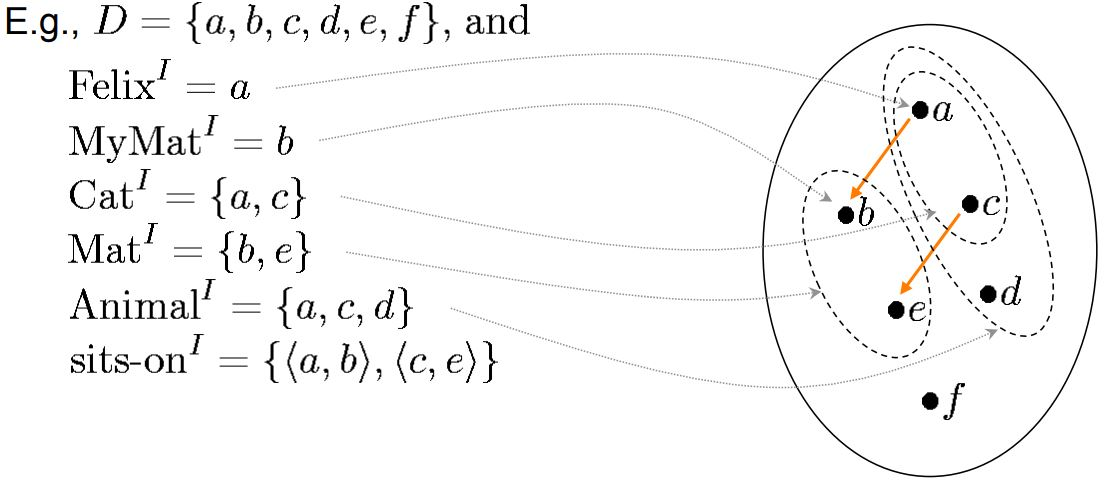
\includegraphics[width=\textwidth]{FOL.JPG}
  \caption{First-order Logic}
  \label{fig:FOL}
\end{figure}

Table \ref{table:FOL_truth_evaluation} shows some truth value evaluation examples in the above given model $M = <D, .^{I}>$, see figure \ref{fig:FOL} for model definition.

\begin{longtable}[h]{ p{100mm} p{30mm} }
\caption{FOL Truth value evaluation}
\label{table:FOL_truth_evaluation}\\
\hline
Statement & Evaluation\\
\hline
$\exists x.Cat(x)$ & true\\
$\forall x.Cat(x)$ & false\\
$\exists x.Cat(x) \land Mat(x)$ & false\\
$\forall x.Cat(x) \rightarrow Animal(x)$ & true\\
$\forall x.Cat(x) \rightarrow (\exists y.Mat(y) \land sits-on(x,y))$ & true\\
\hline
\end{longtable}

\subsubsection{Satisfiability and Decidability}
\label{sec:satisfiability_decidability}

Given a model M and a formula F, M is a model of F (written $M \models F$) iff F evaluates to true in M.
See examples below.

$M \models \exists x.Cat(x)$

$M \not\models \forall x.Cat(x)$

$M \not\models \exists x.Cat(x) \land Mat(x)$

$M \models \forall x.Cat(x) \rightarrow Animal(x)$

$M \models \forall x.Cat(x) \rightarrow (\exists y.Mat(y) \land sits-on(x,y))$

A formula F is \textbf{satisfiable} iff there exists a model M s.t. $M \models F$.

A formula F \textbf{entails} another formula G (written $F \models G$) iff every model of F 
is also a model of G (i.e., $M \models F$ implies $M \models G$). 

Satisfiable examples:

$Cat(Felix) \models \exists x.Cat(x)$

$(\forall x.Cat(x) \rightarrow Animal(x)) \land Cat(Felix) \models Animal(Felix)$

$(\forall x.Cat(x) \rightarrow Animal(x)) \land \neg Animal(Felix) \models \neg Cat(Felix)$

Not satisfiable:

$Cat(Felix) \models \forall x.Cat(x)$

$sits-on(Felix, Mat1) \land sits-on(Tiddles, Mat2) \models \neg sits-on(Felix, Mat2)$

$sits-on(Felix, Mat1) \land sits-on(Tiddles, Mat1) \models \exists^{\geq 2} x.sits-on(x, Mat1)$

Satisfiability in the first-order logic is undecidable, i.e. no algorithm can decide correctly whether a given first-order formula is true or not. However, for any single statement $\varphi$ it is easy to come up with an algorithm that decides $\varphi$ correctly (just hard-code the answer). 
You can encode the statement \textbf{"the Turing machine T halts on empty input"} in first-order logic, this statement is already undecidable, that is, no algorithm can correctly decide whether such a formula is true or not, 
see section \ref{sec:halting_problem} about why. 
Other logics (propositional logic, DL) is decidable because they don't have the power to encode such statement \cite{30672}.

Example decidable fragments: FOL with Counting quantifiers ($\exists^{\geq n}, \exists^{\leq n}$)

$\exists^{\geq 3}x.Cat(x)$ equivalent to

$\exists x,y,z.Cat(x) \land Cat(y) \land Cat(z) \land x \neq y \land x \neq z \land y \neq z $

$\exists^{\leq 2}x.Cat(x)$ equivalent to

$\forall x,y,z.Cat(x) \land Cat(y) \land Cat(z) \rightarrow x=y \lor x=z \lor y=z $

\subsubsection{Halting Problem}
\label{sec:halting_problem}
In computability theory, the halting problem is the problem of determining, from a description of an arbitrary computer program and an input, whether the program will finish running or continue to run forever.

Alan Turing proved in 1936 that a general algorithm to solve the halting problem for all possible program-input pairs cannot exist. A key part of the proof was a mathematical definition of a computer and program, which became known as a Turing machine; the halting problem is undecidable over Turing machines. It is one of the first examples of a decision problem \cite{halting_problem}.

Proof by contradiction:
Suppose that there exists a total computable function \textbf{halts(g)} that returns true if the subroutine g halts (when run with no inputs) and returns false otherwise. Now consider the following subroutine:
\begin{lstlisting}
def g():
    if halts(g):
        loop_forever()
\end{lstlisting}
\textbf{halts(g)} must either return true or false, because halts was assumed to be total. 
If \textbf{halts(g)} returns true, then g will call \textbf{loop\textunderscore forever} 
and never halt, which is a contradiction. 
If \textbf{halts(g)} returns false, then g will halt, 
because it will not call \textbf{loop\textunderscore forever}; this is also a contradiction. 
Overall, \textbf{halts(g)} can not return a truth value that is consistent with whether g halts. 
Therefore, the initial assumption that halts is a total computable function must be false.

\subsection{Knowledge Base}
\label{sec:KB}

A knowledge base (KB) \cite{knowledge_base} is a technology used to store complex structured and unstructured information used by a computer system. A knowledge-based system consists of a knowledge-base that represents facts about the world and an inference engine \cite{jena} that can reason about those facts and use rules and other forms of logic to deduce new facts or highlight inconsistencies.

The term "knowledge-base" was coined to distinguish this form of knowledge store from the more common and widely used term database. At the time (the 1970s) virtually all large Management Information Systems stored their data in some type of hierarchical or relational database. At this point in the history of Information Technology the distinction between a database and a knowledge base was clear and unambiguous. A database had ACID transaction properties: Atomicity, Consistency, Isolation, and Durability. Early expert systems had little need for the complexity that comes with requiring transactional properties on data. 

The volume requirements were also different for a knowledge-base compared to a conventional database. The knowledge-base needed to know facts about the world. For example, to represent the statement that "All humans are mortal". A database typically could not represent this general knowledge but instead would need to store information about thousands of tables that represented information about specific humans. Representing that all humans are mortal and being able to reason about any given human that they are mortal is the work of a knowledge-base. Representing that George, Mary, Sam, Jenna, Mike,... and hundreds of thousands of other customers are all humans with specific ages, sex, address, etc. is the work for a database.

The next evolution for the term knowledge-base was the Internet. With the rise of the Internet, documents, hypertext, and multimedia support were now critical for any corporate database. It was no longer enough to support large tables of data or relatively small objects that lived primarily in computer memory. 

Knowledge Base Consistency Checking:
Given knowledge base K as input, a decision procedure for knowledge base consistency returns “K is consistent” if there is an interpretation I such that $I \models K$, otherwise it returns “K is inconsistent.” \cite{KnowledgeBaseConsistency}, see section \ref{sec:satisfiability_decidability} for more definitions. 

\subsection{Linked Data}

In computing, linked data (often capitalized as Linked Data) is a method of publishing structured data so that it can be interlinked and become more useful through semantic queries. It builds upon standard Web technologies such as HTTP, RDF and URIs, but rather than using them to serve web pages for human readers, it extends them to share information in a way that can be read automatically by computers.

Tim Berners-Lee, director of the World Wide Web Consortium (W3C), coined the term in a 2006 design note about the Semantic Web project \cite{LinkedData}. Linked data may also be open data, in which case it is usually described as linked open data (LOD).

Some example Resource Description Framework serialization formats are RDF/XML, JSON-LD \cite{JSON-LD} . 

Some example Datasets (knowledge base):

\begin{enumerate}
    % 1
    \item 
    DBpedia – a dataset containing extracted data from Wikipedia; it contains about 3.4 million concepts described by 1 billion triples, including abstracts in 11 different languages.
    % 2
    \item
    FOAF \cite{FOAF} – a dataset describing persons, their properties and relationships.
    % 3
    \item
    GeoNames provides RDF descriptions of more than 7,500,000 geographical features worldwide.
     % 4
    \item
    Wikidata – a collaboratively-created linked dataset that acts as central storage for the structured data of its Wikimedia Foundation sister projects.In 2014, Freebase \cite{Freebase} merged into Wikidata, Google's Knowledge Graph was powered in part by Freebase.
\end{enumerate}

\subsection{Schema.org and Google Knowledge Graph}

Schema.org \cite{Schema.org} is an initiative launched on 2 June 2011 by Bing, Google and Yahoo to "create and support a common set of schemas for structured data markup on web pages." In November 2011 Yandex (whose search engine is the largest one in Russia) joined the initiative.

The Knowledge Graph is a knowledge base used by Google and its services to enhance its search engine's results with information gathered from a variety of sources. This information is presented to users in a box to the right of search results. Knowledge Graph boxes were added to Google's search engine in May 2012. The information covered by the Knowledge Graph grew significantly after launch, tripling its original size within seven months, and being able to answer "roughly one-third" of the 100 billion monthly searches Google processed in May 2016 \cite{Knowledge_Graph}.
In October 2016, Google announced that the Knowledge Graph held over 70 billion facts. The information is often used as a spoken answer in Google Assistant and Google Home searches. 

The Knowledge Graph Search API uses standard schema.org types and is compliant with the JSON-LD specification.

The Knowledge Graph has been criticized for providing answers without source attribution.

\subsection{RDF}
\label{sec:RDF}
The purpose of RDF is to provide a structure (aka framework)
for describing identified things (aka resources) \cite{RDFandOWL_SenmanticWebAffinityGroup}.
The RDF data model is based on statements to describe and feature resources, especially web resources, in the form of subject-predicate-object (resource–property–value) expressions (RDF triples) \cite{rdf-triples}.

Structured datasets can be written in RDF using a variety of other syntax notations and data serialization formats, for example, RDFa, JSON-LD, Notation3 (N3), Turtle \cite{rdfTurtle}, etc. The N3 syntax is, for example, less verbose than the RDF/XML serialization. A subset of N3 is the Terse RDF Triple Language, often referred to as Turtle. Turtle provides a syntax to describe RDF graphs in a compact textual form, which is easy to develop. It is a subset of Notation 3 (N3) and a superset of N-Triples. Turtle is popular among Semantic Web developers and considered as an easy-to-read alternative to RDF/XML. The typical file extension of Turtle files is \texttt{.ttl}. The character encoding of Turtle files should be \texttt{UTF-8}. The MIME type of Turtle is \texttt{text/turtle}. Turtle is supported by many software frameworks that can be used for querying and analyzing RDF data, such as Jena and Sesame. Turtle files consist of a sequence of directives, statements representing triples, and blank lines.

\subsection{RDFS}
As mentioned in Section \ref{sec:RDF}, RDF allows you to link resources (concepts) together so you could say that (Karthik  is a person). Think about it as directed graph, however you can't classify objects so you can't say for example that person is a subclass of human-beings.

RDFS (RDF Schema) gives you more expressive vocabulary, this means you can start making statements about classes of thing, and types of relationship. It also allows you to describe in human readable text the meaning of a relationship or a class.
It allows you to classify resources by using the class and subclass (\texttt{rdfs:class}, \texttt{rdfs:subclass}) notions. It also allows you to set restriction on the properties(relationships) using \texttt{rdfs:Domain} and texttt{rdfs:range}.
It tells you legal uses of various classes and relationships. It is also used to indicate that a class or property is a sub-type of a more general type. For example "HumanParent" is a subclass of "Person". "Loves" is a sub-class of "Knows"\cite{RDFvsOWL_SO}.

\subsection{OWL}
The purpose of OWL is to develop ontologies that are compatible with the World Wide Web \cite{RDFandOWL_SenmanticWebAffinityGroup}.
OWL it is closely related to it to RDF, however, OWL is not an extension to RDF, in the same sense that DTDs and XML Schema are not extensions to XML \cite{RDFvsOWLquora}. 
OWL is a way of adding meaning / semantic richness to RDF.  Among other things this allows automated reasoning / influencing.
OWL is a way to define types for RDF data, though OWL "typing"  differs from conventional type systems in that it has an open world  assumption. OWL is represented using RDF triples and typically expressed using RDF/XML syntax.
OWL allows you to add more restrictions. It categorises properties(relationships) into object and data properties and allows you to add restrictions on your properties.

\subsection{Ontology Design Pattern}
Like the software design patterns, many Ontology design patterns(ODP) \cite{ODP}
also have been proposed to suggest standardized solutions for common problems.

\subsection{Related Research}
The research group of the Department of Soft Computing and Intelligent Information Systems
at the University of Granada \cite{DataMiningServicedefinitionInCloud}, 
has developed two small Cloud ontologies.
The set of concepts and features they covered are limited and as a result, their examples are limited to some simple cases.
For instance, the examples presented in Section \ref{sec:PriceSpecification}
can not be modeled with their ontologies.
Since their data-sets link are now inaccessible,
there is no further evidence of the applicability of their model today.

K. Boukadi et al. developed a Cloud Service Description Ontology (CSO) \cite{Boukadi2016CloudSD}, where they model a Cloud Service brokerage. The the price model is overly simplified, compared to real word scenarios. Their model and data is also not available online to evaluate it further or to reuse it in other contexts.

The mOSAIC project \cite{Moscato2011AnAO} proposed an OWL ontology for Cloud services negotiation (i.e. between costumer and provider) and composition (i.e. by an administrator). They have a very different scope.

K. Joshi et al. developed an OWL Ontology for the Lifecycle of IT Services in the
Cloud \cite{Joshi2014AutomatingCS}. It models the steps involved in the
phases of discovery, negotiation, composition, and consumption of Cloud Service.
The Cloud service features modelled are very limited, link to an example of a
storage service \cite{kjoshi_storage_ontology} is no longer accessible.

Overall, these other research projects had different focuses. 
Our focus is on modeling realistic price specifications of cloud service and their  features, 
but models for orchestration \cite{Moscato2011AnAO,Joshi2014AutomatingCS} or
brokerage processes \cite{Boukadi2016CloudSD} are outside of the scope of the proposed ontology. However, our ontology could be extended in this regard using the models proposed in these works.
The rest of the projects \cite{Boukadi2016CloudSD,Moscato2011AnAO}
do not make their model and data available, and hence are not easy to use or to replicate their results and require a significant mapping effort in their adoption (mapping to real service data).
To address the issue of mapping to real word data, we also developed tools for automatically converting data from provider API's to RDF data for our use cases. These mapping tools are also easily extensible to cover scenarios outside the one's presented in this thesis.

\section{Web Service Discovery Techniques}
\label{sec:WebServiceDiscoveryTechniques}
We surveyed a list of state of the art in Service Selection and Comparison techniques, we highlight their significant limitations, their relationship and dependency on some of the prior concepts from other fields in computing. 

\subsection{Historical Web Service Discovery}
There are a lot research in \textbf{web} service discovery. Example products of such research includes \textbf{Semantic Web},  Web Services Description Language (\textbf{WSDL}) and Universal Description, Discovery, and Integration (\textbf{UDDI}). Among those, UDDI has not been as widely adopted as its designers had hoped. It has been closed. On the other hand, Semantic Web is still very active. 

According to the W3C, "The Semantic Web provides a common framework that allows data to be shared and reused across application, enterprise, and community boundaries". The term was coined by Tim Berners-Lee for a web of data that can be processed by machines — that is, one in which much of the meaning is machine-readable. While its critics have questioned its feasibility, proponents argue that applications in industry, biology and human sciences research have already proven the validity of the original concept \cite{SemanticWeb}.

The term "Semantic Web" is often used more specifically to refer to the formats and technologies that enable it. The collection, structuring and recovery of linked data are enabled by technologies that provide a formal description of concepts, terms, and relationships within a given knowledge domain. These technologies are specified as W3C standards and some examples are:

\begin{enumerate}
    % 1
    \item 
    Resource Description Framework (RDF), a general method for describing information.
    % 2
    \item
    SPARQL, an RDF query language.
    % 3
    \item
    Web Ontology Language (OWL), a family of knowledge representation languages. For adding meaning to web content by annotating it with terms defined in ontologies.Supported by tools (e.g. Protégé) and APIs (e.g. OWL API). Based on Description Logics \cite{OntologyLanguageTool2}.
\end{enumerate}

Some of the "Cloud discovery" research just focused on the SaaS and PaaS domain, which I consider mostly can be categorized into web service discovery research. Other research projects may have included IaaS, but have over simplified the billing model or offering types, see section \ref{sec:research_problem} for more details about the complexity of those Cloud IaaS offers, thus impractical for real life scenarios. Some examples are:

\begin{enumerate}
    % 1
    \item  
    Efficient Service Discovery for Cloud Computing Environments
    \cite{EfficientServiceDiscoveryforCloudComputingEnvironments}, 
    semantics-based discovery using ontology and UDDI. Capture Cloud services details features with Web Services Description Language(WSDL) and publishing them on the web service registry (UDDI).
    But UDDI is dead.
    % 2
    \item
    Cloudle \cite{Cloudle, CloudleAgent-BasedCloudComputing}, Cloud services search engine, uses web crawler agent, ontology, k-means clustering algorithm to discover services over the Internet. 
    The proposed system was evaluated using virtual (provider) websites, how well it process real websites is questionable. Besides, Cloud providers still need to register their services in a central database. Also Cloudle's similarity is calculated on very limited number of attributes (10), a real word offer can consist many times more attributes, which may result in inaccurate clustering.
    % 3
    \item
    Integrating intelligent agent and ontology for services discovery on cloud environment
    \cite{IntelligentAgentOntologyServicesDiscovery}, the proposed framework utilizes mobile agents with ontology for searching appropriate services in cloud environment, inference rules are defined and executed by Jena engine \cite{jena} in a mobile reasoner.Mobile agents are implemented using JAVA Agent DEvelopment Framework (JADE).
    Despite the different method for retrieving information, the evaluation does not demonstrate much superiority compare to other researches. It achieves no more than 40 percent recall, means it can only retrieve 40 percent of what should be discovered (with human review).
    % 4
    \item
    OWL-S Based Semantic Cloud Service Broker \cite{OWL-CloudServiceBroker}, semantics OWL-based service broker.
    Shared ontology among cloud providers is needed to be implemented for translating the offered and requested services. QoS parameters are not included.
    % 5
    \item 
    A Cloud computing approach based on mobile agents for Web services discovery
    \cite{MobileAgentsWebServicesDiscovery}, a Keywords-based search implemented using mobile agents.    
    % 6
    \item
    Ontology-based annotation and retrieval of services in the cloud \cite{Ontology-basedAnnotationRetrievalOfServicesInCloud}.
    % 7
    \item
    A Crawler Engine for Cloud Services Discovery on the World Wide Web \cite{CSCE}.
    % 8
    \item
    A semantic-based Software-as-a-Service (SaaS) discovery and selection system \cite{SaaSdiscoverySelectionSystem}.
    % 9
    \item
    Toward dynamic and attribute based publication, discovery and selection for cloud computing \cite{DynamicAttributeBasedPublicationDiscoverySelectionForCloud}, introduced a semantic schema for service publication discovery and selection.
    % 10
    \item
    Semantic Discovery of Cloud Service Catalog Published Over Resource Description Framework \cite{Vasudevan2014SemanticDO}, Semantic Discovery based on RDF.
    % 11
    \item
    Design and Implementation of the Hadoop-Based Crawler for SaaS Service Discovery \cite{Hadoop-BasedCrawlerForSaaSDiscovery}.
    % 12
    \item
    Integrating Software Agents and Web Services in Service Oriented Architecture Based Cloud Services Discovery Framework \cite{AgentSOAServicesDiscovery}.
    % 13
    \item
    A Multi-agent-Based Framework for Cloud Service Description and Discovery Using Ontology \cite{Multi-agent-BasedCloudDescriptionDiscoveryOntology}.
    % 14
    \item
    Automatic Extraction of Metrics from SLAs for Cloud Service Management \cite{AutoExtractionSLA}.
    % 15
    \item
	A Cloud Repository and Discovery Framework Based on a Unified Business and Cloud Service Ontology \cite{CloudRepositoryDiscoveryFrameworkBasedonOntology}.
\end{enumerate}

I have included a summary table about some limitations of the above projects, please see Table \ref{table:related_work} for more details. Overall, projects included in this section do not provide more comprehensive comparison, neither include QoS into comparison. There is no reference to the code base of the implemented systems, it's impossible to reproduce results and little provide evaluation on real word data.

\subsection{IaaS Pricing Calculation}

Although branded calculators are available from individual cloud providers
\cite{AWSCalculator, AzurePricingCalculator, GooglePricingCalculator, RackspaceCalculator, SoftLayerCalculator}
for calculating the service leasing cost, it is not easy for users to
generalize their requirements to fit different service offers (with
various quota and limitations), let alone compute and compare
costs. 

It's hard to do decent comparison, due to the very different nature of what things are part of billing and how they are part of billing. For some, a year consists of 365 days, for others it's only 360. While it is great that Cloud vendors provide an API for pricing estimation and calculation, the very different nature of the offerings themselves make it very hard to compare them \cite{Cloudorado}.

\subsection{Other Commercial Offers} 

The key features distinguish our solution to exiting commercial offers
\cite{BurstormRecommendation, CloudHarmonyProviderDirectory, RightscaleCloudPricingService, Cloudorado, CloudReviews} 
is the application of AHP-based decision making technique
and Queuing Theory based QoS modeling in our algorithm.

\subsection{Research Works}

Swinburne University has a research project called 
Smart Cloud Broker Service \cite{OpenMarketforTradingCloudServices}.
From the screen-cast they released, we can tell that their
benchmarking is done in real time, which means that users
have to wait for the results to come back. We have considered
this kind of situation but decided to collect the benchmarking
result beforehand. This is because this way, no matter how
many cloud providers users want to compare against, they can
still get the result with minimum (or no) waiting time. Another
reason we choose to do it this way is because, at any particular
point in time, the network benchmark result is not conclusive as
performance fluctuates during time; thus, we use an aggregated
average, which is a more reliable overall indication.

Menzel and Ranjan introduced a framework called
“CloudGenius” \cite{CloudGenius} that supports a decision-making process on web
server migration into the cloud. Our system supplements and
partially extends their work. CloudGenius \cite{CloudGenius} focuses on
VM selection, which means that it considers the software requirements
(i.e., the operating system version and the supported
languages), but our study focuses more on the hardware requirements
(i.e., the size of memory and hard disk). Although we
have borrowed the idea of using the AHP (with modification) from CloudGenius,
we used it differently. We have implement the method while following the declarative programming
paradigm, which should be easier to scale out as opposed to rewriting an imperative code implementation.

There are methods proposed for network-aware service composition
\cite{Yu2007, Benatallah2004, Zheng2013}
considering a generic web service, i.e., at the
Software-as-a-Service and Platform-as-a-Service levels. However,
the compatibility constraints at the IaaS level are different
from those at the web service. For example, generic web
services are distinguished by their features, QoS, and prices.
It does not make sense to include two exact same services in
one composition as one job does not need to be done twice, but
using multiple quantities of an IaaS offer is perfectly valid.

\subsection{Summary}

\begin{longtable}{ p{30mm} | p{50mm} | p{50mm} } 
\caption{Related work \label{table:related_work}} \\
\hline
\multicolumn{3}{c}{ \cellcolor{yellow} Fully Automatic Service Discovery Techniques}\\
\hline
\multicolumn{3}{p{140mm}}{All fully automatic techniques facing the same challenge of natural language processing, thus only a limited set of attributes can be captured by the proposed ontologies, and most research can only offer keyword based search, or does not consider service performance.}\\
\hline
Research Title & Proposed Method & Limitation \\ 
\hline
	A semantic-based Software-as-a-Service (SaaS) discovery and selection system \cite{SaaSdiscoverySelectionSystem}. &
    Offers text/term based search. Firstly, Cloud service providers register their services, this data is  processed by consulting the WordNet \cite{WordNet} ontology to expand the service description using the token synonyms, it is  then stored in their proposed ontology. TFIDF algorithm is used to calculate weight vector for each service, then the cosine similarity between those vectors are calculated, finally the agglomerative clustering algorithm is applied to categorize services based on similarity.&
    Despite all the information retrieval techniques applied, it still requires service providers to register themselves manually. \\
\hline
	Semantic Discovery of Cloud Service Catalog Published Over Resource Description Framework \cite{Vasudevan2014SemanticDO} &
    Semantic Discovery based on RDF. String similarity is calculated by Levenshtein (edit) distance. Concept  similarity is calculated by finding the Least Common Hypernym (LCH) in WordNet \cite{WordNet}.The system was implemented with the Jena inference rules engine \cite{jena}.&
    Missing key references such as: which ReVerb did they use, making it hard to evaluate and reproduce the work.\\
\hline
	Integrating intelligent agent and ontology for services discovery on cloud environment
    \cite{IntelligentAgentOntologyServicesDiscovery} & 
    Integrating mobile agents with ontology for searching cloud services
    using inference rules executed by Jena engine \cite{jena}.& 
    Despite the different method for retrieving information, the evaluation does not demonstrate much superiority compare to other researches. It achieves no more than 40 percent recall, means it can only retrieve 40 percent of what should be discovered (with human review).\\ 
\hline
	OWL-S Based Semantic Cloud Service Broker \cite{OWL-CloudServiceBroker}&
    semantics OWL-based service broker.&
    Shared ontology among cloud providers is needed to be implemented for translating the offered and requested services. QoS parameters are not included.\\
\hline
    A Cloud computing approach based on mobile agents for Web services discovery
    \cite{MobileAgentsWebServicesDiscovery}&
    Crawling information using mobile agents, keyword-based search is used to compare between user request and cloud service description.& 
    It does not cover numeric attributes such as cost and performance.\\
\hline
    Ontology-based annotation and retrieval of services in the cloud \cite{Ontology-basedAnnotationRetrievalOfServicesInCloud}&
    Annotates cloud services descriptions in natural language using semantic techniques such as TFIDF (term frequency inverse document frequency algorithm) and ontology (OWL2).&
    It only covers a few attributes. The validation of the system was performed on a small set of services without statistical analysis on large data sets.\\
\hline
	A Crawler Engine for Cloud Services Discovery on the World Wide Web \cite{CSCE} &
    Crawl cloud web portals and store the retrieved Cloud services information in a local repository. The collected Cloud services were categorized into IaaS, PaaS and SaaS based on Ontology.&
    This research is mainly addressing the entry point problem for fully automatic discovery, the data collected from each service are limited, thus there is no mentioning of addressing the more complex need of comparing services, or filter service on certain attributes (price, VM type and RAM or performance).\\
\hline
	Design and Implementation of the Hadoop-Based Crawler for SaaS Service Discovery \cite{Hadoop-BasedCrawlerForSaaSDiscovery}.&
    Hadoop framework \cite{Hadoop} based crawler, implemented with Solr search platform \citet{ApacheSolr}.&
    Do not distinguish between IaaS, PaaS or SaaS. \\
\hline
	Integrating Software Agents and Web Services in Service Oriented Architecture Based Cloud Services Discovery Framework \cite{AgentSOAServicesDiscovery}.&
	Multi agent system for Cloud service discovery and ranking following the Service Oriented Architecture \cite{SOA}. &
    Didn't include design or method on how to implement a system follow the proposed architecture. It is critical because, tasks such as generate taxonomy tree, similarity reasoning, measure documentation and compliance, evaluate client source code, can be very complex subsystem/subproblem on its own, without a concrete ground the proposed system can not be fully realized.\\
\hline
	Automatic Extraction of Metrics from SLAs for Cloud Service Management \cite{AutoExtractionSLA}&
    A prototype system, which automatically extracted the terms defined and measures of SLA documents written in text files. The extracted terms are saved as RDF graph to represent the knowledge base. &
    It covers SAL only. It does not provide a comparison of SLA among different providers.\\
\hline
	CSRecommender \cite{CSRecommender}&
    A search engine system called CSRecommender optimised especially for cloud services. It identifies some interested sites to crawl their web pages,
    a score is assigned to each page based on key word frequencies (i.e. TFIDF is used). It also collected users rating on the search result, to improve the recommendation relevance.&
    It was applied on few cloud services. Accuracy is low. It does not cover all types of Cloud services.\\
\hline
% Semi-automatic Service Discovery 
\multicolumn{3}{c}{\cellcolor{yellow} Semi-automatic Service Discovery with More Complex Filtering}\\
\hline
Research Title & Proposed Method & Limitation \\
\hline
	A Cloud Repository and Discovery Framework Based on a Unified Business and Cloud Service Ontology \cite{CloudRepositoryDiscoveryFrameworkBasedonOntology}&
    A framework that served as a services repository. It provides an integrated, unified business service and cloud ontology to help organizations to discover suitable cloud services using querying abilities. &
    The equalization between the query and business function asked by the user. The SPARQL query language was mainly comprehensive to expert users only. No evaluation on real market data, result only shows a mock-up "Selected Cloud provider".\\
\hline
    A Multi-agent-Based Framework for Cloud Service Description and Discovery Using Ontology \cite{Multi-agent-BasedCloudDescriptionDiscoveryOntology}&
    A prototype system for describing and discovering Cloud services, based on ontology and agents.&
    Requires service provider to implement agent system to interact with service registry. No evaluation with real data.\\
\hline
	Toward dynamic and attribute based publication, discovery and selection for cloud computing \cite{DynamicAttributeBasedPublicationDiscoverySelectionForCloud} &
    A semantic schema extending WSDL, by adding attributes for describing current state of the services, e.g. Amount of free disk space or memory, Number of processes running, percent of CPU used. &
    Because of the tightly coupling with the Web Service SOAP technology stack, there is limited application on its own, SOAP is a bit out dated compare to more recent technologies. \\
\hline   
    Efficient Service Discovery for Cloud Computing Environments
    \cite{EfficientServiceDiscoveryforCloudComputingEnvironments} & 
    Store Cloud service in WSDL file for publishing in an UDDI directory.& 
    UDDI is an old (outdated) technology and abandoned by market and community.\\ 
\hline
	Cloudle \cite{Cloudle, CloudleAgent-BasedCloudComputing} & 
    Uses agents, ontology, k-means clustering algorithm to discover services over the Internet. & 
    Evaluated using virtual (provider) websites. 
    Cloud providers still need to register their services in a central database.
    Cloud ontology only covers limited attributes,
    which will affect the similarity calculated between Cloud services.\\ 
\hline
% Web service composition 
\multicolumn{3}{c}{ \cellcolor{yellow} Web Service Composition}\\
\hline
\multicolumn{3}{p{140mm}}{There are methods proposed for network-aware service composition
\cite{Yu2007, Benatallah2004, Zheng2013}
considering generic web services, i.e., at the
Software-as-a-Service and Platform-as-a-Service levels. However,
the compatibility constraints at the IaaS level are different
from those at the web service. For example, generic web
services are distinguished by their features, QoS, and prices.
It does not make sense to include two exact same services in
one composition as one job does not need to be done twice, but
using multiple quantities of an IaaS offer is perfectly valid.}\\
\hline
% Cloud IaaS 
\multicolumn{3}{c}{ \cellcolor{yellow} Cloud IaaS Selection}\\
\hline
\multicolumn{3}{c}{Providers' Calculators}\\
\hline
\multicolumn{3}{p{140mm}}{Although branded calculators are available from individual cloud providers
\cite{AWSCalculator, AzurePricingCalculator, GooglePricingCalculator, RackspaceCalculator, SoftLayerCalculator}
for calculating the service leasing cost, it is not easy for users to
generalize their requirements to fit different service offers (with
various quota and limitations), let alone compute and compare
costs. It's hard to do decent comparison, due to the very different nature of what things are part of billing and how they are part of billing. For some, a year consists of 365 days, for others it's only 360. While it is great that Cloud vendors provide an API for pricing estimation and calculation, the very different nature of the offerings themselves make it very hard to compare them \cite{Cloudorado}.}\\
\hline
\multicolumn{3}{c}{Commercial Offers}\\
\hline
\multicolumn{3}{p{140mm}}{
Existing commercial offers
\cite{BurstormRecommendation, CloudHarmonyProviderDirectory, RightscaleCloudPricingService, Cloudorado, CloudReviews}
are different to our solution in 3 aspects:
ontology based knowledge representation;
the application of AHP-based decision making technique;
the Queuing Theory based QoS modeling algorithm.}\\
\hline
\multicolumn{3}{c}{Research}\\
\hline
Research Title & Proposed Method & Limitation \\ 
\hline
    An automated approach to cloud storage service selection \cite{Ruiz-AlvarezCloudStorageSelection}&
    Cloud storage service (IaaS level) representation using XML.&
    This research only focused on Storage.
    The proposed schema does not comply with or take into account any existing standards. We believe that semantic web technologies should be adopted to standardize the Cloud services representations.\\
\hline
    An Open Market for Trading Cloud Services \cite{OpenMarketforTradingCloudServices}&
    This research focus on the Cloud markets trading/brokerage potential mechanism. &
    Their benchmarking is done in real time, which means that users
    have to wait a long time for the results to come back.
    At any particular point in time, the network benchmark result is not conclusive as performance may fluctuates during time.
    Our work used average of continuously collected data.\\
\hline
    CloudGenius \cite{CloudGenius} &
    This research focuses on VM and image selection,
    it considers the software requirements
    (i.e., the operating system version and the supported
    languages) &
    Our study focuses more on the hardware requirements
    which also includes hard disks and networks.\\
\hline
\end{longtable}

\section{Multiple-criteria decision analysis}
\label{sec:MCDA}
Multiple-criteria decision-making (MCDM) or multiple-criteria decision analysis (MCDA) is a sub-discipline of operations research that explicitly evaluates multiple conflicting criteria in decision making (both in daily life and in settings such as business, government and medicine). Conflicting criteria are typical in evaluating options: cost or price is usually one of the main criteria, and some measure of quality is typically another criterion, easily in conflict with the cost \cite{MCDA}.

MCDM problems are usually subdivided into continuous and discrete types. MCDM problems have two classifications: Multiple Objective Decision-making (MODM) and Multiple Attribute Decision-making (MODM). MODM methods have decision variables values that are determined in a continuous or integer domain, with a large number of alternative choices. MADM methods are generally discrete, with limited number of pre-specified alternatives. Each decision matrix has four main parts, namely: (a) alternatives, (b) attributes, (c) weight or relative importance of each attribute and (d) measures of performance of alternatives with respect to the attributes\cite{MCDM}. 
Of the many MADM methods, five methods are commonly used: Simple Additive Method (SAW), Weighted Product Method(WPM), Analytical Hierarchy Process (AHP), Techniques for Order Preference by Similarity to Identical Solution (TOPSIS), a Compromise ranking method (VIKOR).

\subsection{Simple Additive Weighting(SAW) Method}
SAW method is based on the weighted average. An evaluation score is calculated for each alternative by multiplying the scaled value given to the alternative of that attribute with the weights of relative importance directly assigned by decision maker followed by summing of the products for all criteria. The advantage of this method is that it is a proportional linear transformation of the raw data which means that the relative order of magnitude of the standardized scores remains equal \cite{SAW}. 

For example, when calculate ranking with SAW, firstly,
criterion matrix with different unit of measure need to be normalized,
then they are multiplied with weights.
As illustrated in Fig. \ref{fig:SAW}, suppose "Loss of life" is considered more important, i.e. given higher weight of 0.6.
"Cultural loss" has a weight of 0.1, "Economic loss" has a weight of 0.3.
After we multiply corresponding weight with each value in the standardized criterion matrix, we get the weighted criterion matrices.
Next sum up all matrices to get one aggregated matrix.
Order values from high to low, the position in the descending list is the final
ranking position, i.e. 1st is the highest value option. As shown in the figure,
the final ranking table contains the order of value from first to the tenth.

\begin{figure}[ht]
  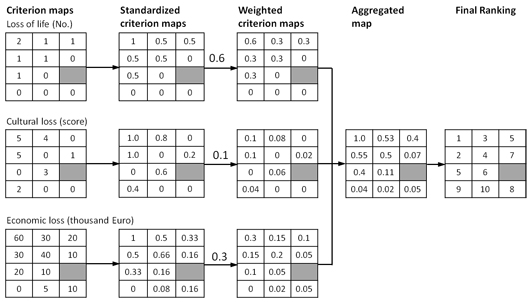
\includegraphics[width=\textwidth]{Figures/background/04_saw_method_web.jpg}
  \caption{SAW example \cite{SAWillustration}}
  \label{fig:SAW}
\end{figure}

\subsection{Weighted Product Method (WPM)}
This method is similar to SAW.
The main difference is that, instead of addition in the model, there is multiplication. The normalized values are calculated as explained under the SAW method \cite{WPM}. 

For example if we have the 3 alternatives each with 4 criteria as shown in
Table \ref{table:WPM_data}.
\begin{table}
\caption{Example alternatives \label{table:WPM_data}} 
\begin{center}
\begin{tabular}{ c c c c c }
\hline
&	Criteria1 &	Criteria2 &	Criteria3 &	Criteria4 \\
\hline
Weight &	0.20 &	0.15 &	0.40 &	0.25\\
\hline
Alternative1 &	25 &	20 &	15 &	30\\
Alternative2 &	10 &	30 &	20 &	30\\
Alternative3 &	30 &	10 &	30 &	10\\
\hline
\end{tabular}
\end{center}
\end{table}
WPM compare alternatives by computing a P value, like illustrated below:
$$
P(Alternative1/Alternative2)=
(\frac{25}{10})^{0.20}
*(\frac{20}{30})^{0.15}
*(\frac{15}{20})^{0.40}
*(\frac{30}{30})^{0.25}
=1.007 > 1
$$
Similarly, we also get:
$$
P(Alternative1/Alternative3)=1.067 > 1
$$
$$
P(Alternative2/Alternative3)=1.059 > 1
$$
Therefore, the best alternative is Alternative1, since it is superior to all the other alternatives. Furthermore, the following ranking of all three alternatives is as follows: A1 > A2 > A3.

It is worth noting that a useful way of choosing
between an additive score function and a multiplicative one is to consider
whether one is willing to keep giving up or trading off units of one attribute
in exchange for some units of the other attribute, at
a given fixed exchange rate, even to the point where
one has zero of the first attribute. 
If this is not acceptable to the decision maker, then the additive score
function is not appropriate. Likewise, if one does not
believe the exchange rate should stay the same however high or low the attributes levels, then again an additive score function is not suitable \cite{AddorMultiply}.
For example, the UNDP (United Nations Development Programme)
publishes an annual ranking of nations known as the
\href{http://hdr.undp.org}{Human Development Index},
which is very influential and is used by first world
nations to guide their aid allocations.
It is also used by pharmaceutical companies to decide which countries should receive discounted prices.
This index is an aggregate of three criteria: life expectancy, education, and gross national income per capita.
For many years the aggregation was carried out using additive weighting.
This was criticised because this assumed that the criteria were perfectly substitutable. Consequently, the UNDP chose to
change its methodology, and the index
is now calculated using a multiplicative scheme.

\subsection{Analytical Hierarchy Process (AHP)}
One of the most popular analytical techniques for
complex decision-making problems is the analytical hierarchy process \cite{MCDM}.
AHP decomposes a decision-making problem into a system of hierarchies of objectives, attributes and alternatives. An AHP hierarchy can have as many levels as needed to fully characterize a particular decision situation. A number of functional characteristics make AHP a useful methodology. These include the ability to handle decision situations involving subjective judgments, multiple decision makers and the ability to provide measures of consistency of preference. Designed to reflect the way people actually think, AHP continues to be the most highly regarded and widely used decision-making method. AHP can efficiently deal with tangible as well as non-tangible attributes, especially where the subjective judgments of different individuals constitute an important part of the decision process.

\subsubsection{The Revised Analytic Hierarchy Process}
Belton and Gear \cite{revisedAHP} propose a revised version
of the AHP model. They demonstrate that an inconsistency can occur when the AHP is used. A numerical example is presented that consists of three criteria and three alternatives. The indication of the best alternative changes when an identical alternative to one of the non-optimal alternatives are introduced now creating four alternatives. According to the authors, the root for that inconsistency is the fact that the relative values for each criterion sum up to one. Instead of having the relative values of the alternatives sum up to one, they propose to divide each relative value by the maximum value of the relative values.

For example, the original step normalise eigenvector into:
$$\begin{bmatrix}
\frac{1}{11} \\
\frac{9}{11} \\
\frac{1}{11}
\end{bmatrix}$$

The revised method would normalise those to:
$$\begin{bmatrix}
\frac{1}{9} \\
1 \\
\frac{1}{9}
\end{bmatrix}$$

\subsection{Technique for Order Preference by Similarity to Identical Solution (TOPSIS)}
This method is based on the concepts that the chosen alternative should have the shortest Euclidean distance from ideal solution and the farthest from negative ideal solution \cite{MCDM}. The ideal solution is a hypothetical solution for which all attribute values corresponds to the maximum attribute values comprising the satisfying solutions; the negative ideal solution is the hypothetical solution for which all attribute values corresponds to the minimum attribute values.
TOPSIS thus gives a solution that is not only closest to the hypothetically best, that is also the farthest from hypothetically worst.

TOPSIS can suffer from ranking abnormality \cite{SAWvsTOPSIS}.
Ranking abnormality means that the ranking of candidate networks changes when low ranking alternative is removed from the candidate list.

\subsection{Compromise Ranking method (VIKOR)}
The VIKOR method of compromise ranking determines a compromise solution, providing a maximum "group utility" for the majority and a minimum of an "individual regret" for the "opponent"\cite{VIKORformula} .

The MCDM problem is stated as follows: Determine the best (compromise) solution in multicriteria sense from the set of J feasible alternatives $A_{1}, A_{2}$ \textellipsis $A_{J}$, evaluated according to the set of n criterion functions. The input data are the elements $f_{ij}$ of the performance (decision) matrix, where $f_{ij}$ is the value of the i-th criterion function for the alternative $A_{j}$.

The VIKOR procedure has the following steps \cite{VIKOR_method_wiki}:
\begin{enumerate}
    \item Determine the best $f_{i}^{*}$ and the worst $f_{i}^{-}$ values of all criterion functions, i = 1,2,...,n; if the i-th function is benefit:
    $$f_{i}^{*} =  \max\limits_{j} f_{ij} , f_{i}^{-} = \min\limits_{j} f_{ij}$$
    If the i-th function is cost:
    $$f_{i}^{*} = \min\limits_{j} f_{ij} ,f_{i}^{-} = \max\limits_{j} f_{ij}$$
    \item Compute the values $S_{j}$ and $R_{j}$, j=1,2,...,J, by the relations: 
    
    Weighted and normalized Manhattan distance:
    $$S_{j}=\sum_{i=1}^{n} w_{i} \frac{f_{i}^{*} - f_{ij}}{f_{i}^{*} - f_{i}^{-}}$$
    Weighted and normalized Chebyshev distance:
    $$R_{j}=\max\limits_{i} w_{i} \frac{f_{i}^{*} - f_{ij}}{f_{i}^{*} - f_{i}^{-}}$$
    where $w_{i}$ are the weights of criteria, expressing their relative importance.
    \item Compute the values $Q_{j}$, j=1,2,…,J, by the relation
    $$Q_{j} = v \frac{S_{j}-S^{*}}{S^{-}-S^{*}} + (1-v)\frac{R_{j}-R^{*}}{R^{-}-R^{*}}$$
    where 
    $$ S^{*} = \min\limits_{j} S_{j},
    S^{-} = \max\limits_{j} S_{j} $$
    $$ R^{*} = \min\limits_{j} R_{j},
    R^{-} = \max\limits_{j} R_{j} $$
    and v is introduced as a weight for the strategy of maximum group utility, whereas 1-v is the weight of the individual regret.
    \item Rank the alternatives, sorting by the values S, R and Q, from the minimum value. The results are three ranking lists.
    \item Propose as a compromise solution the alternative A(1) which is the best ranked by the measure Q (minimum) if the following two conditions are satisfied:
    \begin{enumerate}
        \item C1: “Acceptable Advantage”: $Q(A_{2})-Q(A_{1}) >= DQ$
        where: $A_{2}$ is the alternative with second position in the ranking list by Q; $DQ = \frac{1}{J-1}$, J is the number of alternatives.
        \item C2: “Acceptable Stability in decision making”: The alternative $A_{1}$ must also be the best ranked by S or/and R. This compromise solution is stable within a decision making process, which could be the strategy of maximum group utility (when v > 0.5 is needed), or “by consensus” v about 0.5, or “with veto” v < 0.5).
    \end{enumerate}
    If one of the conditions is not satisfied, then a set of compromise solutions is proposed, which consists of:
    \begin{enumerate}
        \item Alternatives $A_{1}$ and $A_{2}$ if only the condition C2 is not satisfied, or
        \item Alternatives $A_{1},A_{2}$,...,$A_{M}$ if the condition C1 is not satisfied; $A_{M}$ is determined by the relation $Q(A_{M})-Q(A_{1}) < DQ$ for maximum M (the positions of these alternatives are “in closeness”).
    \end{enumerate}
\end{enumerate}

The obtained compromise solution could be accepted by the decision makers because it provides a maximum utility of the majority (represented by min S), and a minimum individual regret of the opponent (represented by min R). The measures S and R are integrated into Q for compromise solution, the base for an agreement established by mutual concessions.

\subsection{Preference Ranking Organization Method for Enrichment Evaluation (PROMETHEE)}
The Preference Ranking Organization METHod for Enrichment of Evaluations and its descriptive complement geometrical analysis for interactive aid are better known as the Promethee and Gaia methods \cite{Promethee}.
The descriptive approach, named Gaia, allows the decision maker to visualize the main features of a decision problem: he/she is able to easily identify conflicts or synergies between criteria, to identify clusters of actions and to highlight remarkable performances.
The prescriptive approach, named Promethee, provides the decision maker with both complete and partial rankings of the actions \cite{PROMETHEE_MLwiki}.

While it can be used by individuals working on straightforward decisions, the Promethee Gaia method is most useful where groups of people are working on complex problems, especially those with several multi-criteria, involving a lot of human perceptions and judgments, whose decisions have a long-term impact. It has unique advantages when important elements of the decision are difficult to quantify or compare, or where collaboration among departments or team members are constrained by their different specializations or perspectives.

\subsection{Decision-making paradox}
The decision-making paradox arises from the quest for determining reliable decision-making methods.
To find the best decision-making method a decision problem needs to be formulated, for which different decision-making methods are the alternatives. 
Since in the beginning it was assumed that the best method is not known, the problem of selecting the best method was solved by successively using different methods. The methods used in that study \cite{DecisionMakingParadox} were the weighted sum model (WSM), the weighted product model (WPM), and two variants of the analytic hierarchy process (AHP). It was found that when a method was used, say method X (which is one of the previous four methods), the conclusion was that another method was best (say, method Y). When method Y was used, then another method, say method Z, was suggested as being the best one, and so on.

The study \cite{DecisionMakingParadox} demonstrates that it is impossible to determine precisely the best decision-making method, for to do so one needs to use the best decision-making method! This problem of finding the best decision-making method always reaches a Decision-Making Paradox. However, the results of this study recommend that for most of the cases of different weights of the two evaluative criteria the revised AHP appears to be the best decision-making method of the four examined, while the original AHP, appears to be the most inaccurate one.
